\documentclass[12pt,a4paper]{article}
\usepackage[top=1.5cm, bottom=1.5cm, left=2.0cm, right=1.5cm] {geometry}
\usepackage{amsmath,amssymb,fontawesome}
\usepackage{tkz-euclide}
\usepackage{setspace}
\usepackage{lastpage}

\usepackage{tikz,tkz-tab}
%\usepackage[solcolor]{ex_test}
\usepackage[dethi]{ex_test} % Chỉ hiển thị đề thi
%\usepackage[loigiai]{ex_test} % Hiển thị lời giải
%\usepackage[color]{ex_test} % Khoanh các đáp án
\usetikzlibrary{shapes.geometric,arrows,calc,intersections,angles,quotes,patterns,snakes,positioning}
\everymath{\displaystyle}

\def\colorEX{\color{purple}}
%\def\colorEX{}%Không tô màu đáp án đúng trong tùy chọn loigiai
\renewtheorem{ex}{\color{violet}Câu}
\renewcommand{\FalseEX}{\stepcounter{dapan}{{\bf \textcolor{blue}{\Alph{dapan}.}}}}
\renewcommand{\TrueEX}{\stepcounter{dapan}{{\bf \textcolor{blue}{\Alph{dapan}.}}}}

%---------- Khai báo viết tắt, in đáp án
\newcommand{\hoac}[1]{ %hệ hoặc
    \left[\begin{aligned}#1\end{aligned}\right.}
\newcommand{\heva}[1]{ %hệ và
    \left\{\begin{aligned}#1\end{aligned}\right.}

%Tiêu đề
\newcommand{\tenso}{iMath}
\newcommand{\tentruong}{0974.940.049}
\newcommand{\tenkythi}{ĐỀ ÔN TẬP}
\newcommand{\tenmonthi}{Môn học: TOÁN 10}
\newcommand{\thoigian}{}
\newcommand{\tieude}[1]{
    \noindent
     \begin{minipage}[b]{6cm}
    \centerline{\textbf{\fontsize{11}{0}\selectfont \tenso}}
    \centerline{\fontsize{11}{0}\selectfont \tentruong}  
  \end{minipage}\hspace{1cm}
  \begin{minipage}[b]{11cm}
    \centerline{\textbf{\fontsize{11}{0}\selectfont \tenkythi}}
    \centerline{\textbf{\fontsize{11}{0}\selectfont \tenmonthi}}
    \centerline{\textit{\fontsize{11}{0}\selectfont Thời \underline{gian làm bài: \thoigian  } phút }}
  \end{minipage}
  \vspace*{3mm}
  \noindent
  \begin{minipage}[t]{12cm}
    \textbf{Họ, tên thí sinh:}\dotfill\\
    \textbf{Số báo danh:}\dotfill
  \end{minipage}\hfill
  \begin{minipage}[b]{3cm}
    \setlength\fboxrule{1pt}
    \setlength\fboxsep{3pt}
    \vspace*{3mm}\fbox{\bf Mã đề thi #1}
  \end{minipage}\\
}

\newcommand{\chantrang}[2]{\rfoot{Trang \thepage $-$ Mã đề #2}}
\pagestyle{fancy}
\fancyhf{}
\renewcommand{\headrulewidth}{0pt} 
\renewcommand{\footrulewidth}{0pt}

\begin{document}
%Thiết lập giãn dọng 1.5cm 
%\setlength{\lineskip}{1.5em}



%Nội dung trắc nghiệm bắt đầu ở đây


\tieude{159}
\chantrang{\pageref{LastPage}}{159}
\setcounter{page}{1}
{\bf PHẦN I. Câu trắc nghiệm nhiều phương án lựa chọn.}
\setcounter{ex}{0}
\Opensolutionfile{ans}[ans/ans159-1]
\begin{ex}
 Tìm tọa độ đỉnh ${I}$ của đồ thị hàm số $y=- 2 x^{2} + 4 x - 5$.
\choice
{ \True ${I\left(1;-3\right)}$ }
   { ${I\left(-1;-11\right)}$ }
     { ${I\left(2;-5\right)}$ }
    { ${I\left(-2;-21\right)}$ }
\loigiai{ 

 Đồ thị hàm số $y=- 2 x^{2} + 4 x - 5$ có tọa độ đỉnh là ${I\left(1;-3\right)}$.  
 }\end{ex}

\begin{ex}
 Cho hàm số $f(x)=x^{2} + x - 1$. Tính $f(1)$.

 
\choice
{ $ {5 }$ }
   { $ {6}$ }
     { $ {-1}$ }
    { \True ${ 1 }$ }
\loigiai{ 

 Thay giá trị $1$ và hàm số $f(x)=x^{2} + x - 1$ ta được $f(1)=1$. 
 }\end{ex}

\begin{ex}
 Cho hàm số $y=- 3 x^{2} - 5 x - 4 $. Hàm số nghịch biến trên khoảng nào trong các khoảng sau.
\choice
{ $\left(-\infty; +\infty\right)$ }
   { \True $\left(- \frac{5}{6} ; +\infty\right)$ }
     { $\left(-\infty; -1\right)$ }
    { $\left(-\infty; - \frac{5}{6}\right)$ }
\loigiai{ 

  Hàm số nghịch biến trên khoảng $\left(- \frac{5}{6} ; +\infty\right)$. 
 }\end{ex}

\begin{ex}
 Cho hàm số $f(x)=\left\{ \begin{array}{l} 
     x^{2} + 6 x + 2 \text{ khi } x \ge 4  \\ 
     6 x - 5 \text{          khi  } x < 4  
     \end{array} \right.$. Tính $f(-1)$.

 
\choice
{ $ {-3 }$ }
   { \True ${ -11 }$ }
     { $ {1}$ }
    { $ {9}$ }
\loigiai{ 

 Vì $-1<4$ nên thay giá trị $-1$ và hàm số $f(x)=6 x - 5$ ta được $f(-1)=-11$. 
 }\end{ex}

\begin{ex}
 Tìm tập xác định của hàm số $y=\sqrt{x} - \sqrt{8 - 5 x}$.
\choice
{ ${D=\left[0 ;+\infty\right)}$ }
   { \True ${D=\left[0 ;\frac{8}{5} \right]}$ }
     { ${D=\left(-\infty;\frac{8}{5}\right]}$ }
    { ${D=\left(0 ;\frac{8}{5} \right)}$ }
\loigiai{ 

 Điều kiện xác định: .
$\left\{ \begin{array}{l}
            x\ge 0 \\ 
            8 - 5 x\ge 0 
\end{array} \right.$$\Rightarrow\left\{ \begin{array}{l}
            x\ge 0 \\ 
            x\le \frac{8}{5} 
\end{array} \right.$Tập xác định là: ${D=\left[0 ;\frac{8}{5} \right]}$. 
 }\end{ex}

\begin{ex}
 Tìm tập xác định của hàm số $y=\dfrac{4 - 2 x}{3 - 8 x}$.
 
\choice
{ $D=\mathbb{R} \backslash \{ - \frac{3}{8} \}$ }
   { $D=\left( -\infty ; \frac{3}{8} \right)$ }
     { \True $D=\mathbb{R} \backslash \{ \frac{3}{8} \}$ }
    { $D=\left( \frac{3}{8} ; +\infty \right)$ }
\loigiai{ 

 Hàm số xác định khi $3 - 8 x\ne 0 \Leftrightarrow x \ne \frac{3}{8}$. 
 }\end{ex}

\Closesolutionfile{ans}
{\bf PHẦN II. Câu trắc nghiệm đúng sai.}
\setcounter{ex}{0}
\Opensolutionfile{ans}[ans/ans159-2]
\begin{ex}
 Cho hàm số $f(x)=- 4 x^{2} - 2 x - 8$. Xét tính đúng sai của các khẳng định sau.
\choiceTF
{ \True Tập xác định của hàm số là $\mathbb{R}$ }
   { \True Đồ thị hàm số đi qua điểm $D(-4;-64)$ }
     { Hàm số đồng biến trên khoảng $\displaystyle \left(- \frac{1}{4};+\infty \right)$ }
    { Đồ thị hàm số có hoành độ đỉnh là $\displaystyle x_0=\frac{3}{4}$ }
\loigiai{ 
 a) Tập xác định của hàm số là $\mathbb{R}$ là khẳng định đúng vì đây là hàm số đa thức.\\ 
b) Đồ thị hàm số đi qua điểm $D(-4;-64)$ là khẳng định đúng vì có $f(-4)=-64$.\\ 
c) Hàm số đồng biến trên khoảng $\displaystyle \left(- \frac{1}{4};+\infty \right)$ là khẳng định sai vì Hàm số đồng biến trên khoảng $\displaystyle \left(- \frac{1}{4};+\infty \right)$.\\ 
d) Đồ thị hàm số có hoành độ đỉnh là $\displaystyle x_0=\frac{3}{4}$ là khẳng định sai vì hoành độ đỉnh là $\displaystyle x_0=- \frac{1}{4}$.\\ 
 
 }\end{ex}

\begin{ex}
 Cho parabol $(P):y=ax^2+bx=c,(a\ne 0)$ có bảng biến thiên như hình dưới đây. 
\begin{center}
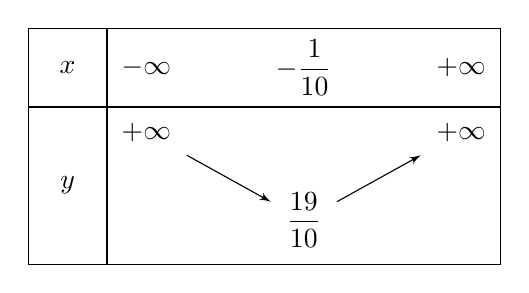
\begin{tikzpicture} 
                \tkzTabInit[nocadre=false, lgt=1, espcl=2] 
                {$x$ /1,$y$ /2}
                {$-\infty$, $\displaystyle - \frac{1}{10}$, $+\infty$} 
                \tkzTabVar{+/$+\infty$ , -/ $\displaystyle \frac{19}{10}$ /, +/$+\infty$ /} 
                \end{tikzpicture}

\end{center}
Xét tính đúng sai của các khẳng định sau:\choiceTF
{ \True Đồ thị hàm số nhận đường thẳng $\displaystyle x=- \frac{1}{10}$ làm trục đối xứng }
   { \True Hàm số có hệ số $a>0$ }
     { \True Trên khoảng $\displaystyle \left(\frac{29}{10};+\infty \right)$ thì hàm số đồng biến }
    { Đồ thị hàm số có tung độ đỉnh bằng $\displaystyle - \frac{1}{10}$ }
\loigiai{ 
 a) Đồ thị hàm số nhận đường thẳng $\displaystyle x=- \frac{1}{10}$ làm trục đối xứng là khẳng định đúng.\\ 
b) Dựa vào dáng của bảng biến thiên, hàm số có hệ số $a>0$ là khẳng định đúng.\\ 
c) Hàm số đồng biến trên khoảng $\displaystyle \left(\frac{29}{10};+\infty \right)$ là khẳng định đúng.\\ 
d) Đồ thị hàm số có tung độ đỉnh bằng $\displaystyle - \frac{1}{10}$ là khẳng định sai vì tung độ đỉnh là $\displaystyle \frac{19}{10}$.\\ 
 
 }\end{ex}

\begin{ex}
 Cho tam giác ${ABC}$ có $c=5,a=5,b=3$. Xét tính đúng-sai của các khẳng định sau.
\choiceTFt
{ $\cos C=\frac{3}{20}$ }
   { $S=\frac{3 \sqrt{14}}{4}$ }
     { $\widehat{A}=81,37^\circ$ }
    { $r=\frac{3 \sqrt{91}}{52}$ }
\loigiai{ 
 

 a) Khẳng định đã cho là khẳng định sai.

 $\cos C=\dfrac{5^2+3^2-5^2}{2.5.3}=\frac{3}{10}$.

b) Khẳng định đã cho là khẳng định sai.

 $p=\dfrac{5+5+3}{2}=\frac{13}{2}$.

$S=\sqrt{\frac{13}{2}.(\frac{13}{2}-5).(\frac{13}{2}-5).(\frac{13}{2}-3)}=\frac{3 \sqrt{91}}{4}$.


c) Khẳng định đã cho là khẳng định sai.

 $\cos A=\dfrac{5^2+3^2-5^2}{2.5.3}=\frac{3}{10} \Rightarrow \widehat{A}=72,54^\circ$.

d) Khẳng định đã cho là khẳng định sai.

 $r=\dfrac{S}{p}=\dfrac{\frac{3 \sqrt{91}}{4}} {\frac{13}{2}}=\frac{3 \sqrt{91}}{26}$.

 
 }\end{ex}

\Closesolutionfile{ans}
{\bf PHẦN III. Câu trắc nghiệm trả lời ngắn.}
\setcounter{ex}{0}
\Opensolutionfile{ans}[ans/ans159-3]
\begin{ex}
 Biết đồ thị hàm số $y=ax^2- x+c$ đi qua các điểm $B(-5;-42)$ và $I(4;-33)$. Tính $P=2 a - 2 c$.


\shortans[4]{-10}

\loigiai{ 
 Đồ thị hàm số đi qua $B(-5;-42)$ và $I(4;-33)$ nên ta có:

$\left\{ \begin{array}{l} 
        25 a + c + 5=-42 \\ 
        16 a + c - 4=-33
        \end{array} \right.$$\Rightarrow \left\{ \begin{array}{l} 
        25 a + c=-47 \\ 
        16 a + c=-29
        \end{array} \right.$$\Rightarrow \left\{ \begin{array}{l} 
        a=-2 \\ 
        c=3
        \end{array} \right.$

$P=2 a - 2 c=-10$. 
 }\end{ex}

\begin{ex}
 Một quả bóng được cầu thủ sút lên rồi rơi xuống theo quỹ đạo là một parabol. Biết rằng ban đầu quả bóng được sút lên từ độ cao 0,4 m, sau đó 1 giây quả bóng đạt độ cao $\frac{12}{25}$ m và sau 4,5 giây quả bóng đạt độ cao $\frac{13}{100}$ m. Hỏi độ cao cao nhất mà quả bóng đạt được là bao nhiêu mét (kết quả làm tròn đến hàng phần mười)?


\shortans[4]{0,5}

\loigiai{ 
 Giả sử $h(t)=at^2+bt+c$ là độ cao của quả bóng theo thời gian ${t}$.

$\left\{ \begin{array}{l} 
    h(0)=0,4 \\ 
    h(1)=\frac{12}{25}\\ 
    h(4,5)=\frac{13}{100}
    \end{array} \right.$$\left\{ \begin{array}{l} 
    c=0,4 \\ 
    a.1^2+b.1+0,4=\frac{12}{25}\\ 
    a.4,5^2+b.4,5+0,4=\frac{13}{100}
    \end{array} \right.$ 
$\Rightarrow \left\{ \begin{array}{l} 
    a=- \frac{1}{25} \\ 
    b=\frac{3}{25} \\ 
    c=\frac{2}{5}
    \end{array} \right.$

$h(t)=- \frac{1}{25}t^2+\frac{3}{25}t+\frac{2}{5}$.

Độ cao của quả bóng đạt được bằng $h_{max}=\frac{49}{100}=0,5$ m khi $t=\frac{3}{2}$. 
 }\end{ex}

\begin{ex}
 Biết đồ thị hàm số $y=- x^{2}+bx+c$ có đỉnh là điểm $I(- \frac{5}{2};\frac{13}{4})$. Tính $P=b + c$.


\shortans[4]{-8}

\loigiai{ 
 Đồ thị hàm số đi qua $A(4;-39)$ và $H(1;-9)$ nên ta có:

$\left\{ \begin{array}{l} 
        4 b + c - 16=-39 \\ 
        \frac{b}{2}=- \frac{5}{2}
        \end{array} \right.$$\Rightarrow \left\{ \begin{array}{l} 
        4 b + c=-23 \\ 
        b=-5
        \end{array} \right.$$\Rightarrow \left\{ \begin{array}{l} 
        b=-5 \\ 
        c=-3
        \end{array} \right.$

$P=b + c=-8$. 
 }\end{ex}

\begin{ex}
 Một mô hình mô phỏng cây cầu treo có trụ tháp đôi cao $BD=AC=\frac{128}{5}$ m và cách nhau $AB=16$ m. Các dây cáp có dạng đồ thị là một Parabol như hình. Một dây nối hai điểm ${M}$ và ${N}$ trên dây cáp như hình. Biết dây nối cách mặt của cây cầu là ${\frac{18}{5}}$. Người ta muốn chăng một đoạn dây đèn trang trí nối thẳng từ điểm ${A}$ đến ${M}$ đến ${N}$ đến ${B}$. Chiều dài đoạn dây đèn là bao nhiêu. (Chỉ làm tròn kết quả cuối cùng đến chữ số thập phân thứ nhất) \ 
\begin{center}

        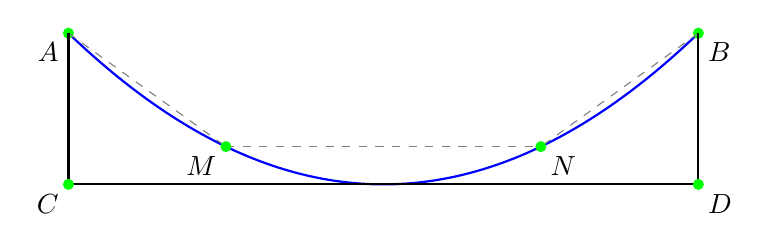
\begin{tikzpicture}
            
            % Vẽ parabol
            \draw[thick, blue] 
            plot[domain=-4:4, samples=100] (\x, {0.12*\x*\x}); % Parabol y = -0.5x^2 + 4
            % Đánh dấu và ghi nhãn hai chân cổng
            \fill[green] (-4, 1.92) circle(2pt); % Chân trái (x = -sqrt(8))
            \node[below left] at (-4, 1.92) {\( A \)}; % Nhãn chân trái là A
            
            \fill[green] (4, 1.92) circle(2pt); % Chân phải (x = sqrt(8))
            \node[below right] at (4, 1.92) {\( B \)}; % Nhãn chân phải là B
            
            % Nối hai chân cổng bằng nét đứt
                \draw[dashed, gray] (-4, 1.92) -- (-2, 0.48);
                    \draw[dashed, gray] (4, 1.92) -- (2, 0.48);  % 
            \draw[thick](-4, 0) -- (4, 0); %
            \draw[thick](-4, 0) -- (4, 0); % 
                \draw[thick](-4, 1.92) -- (-4, 0); %
                \draw[thick](4, 1.92) -- (4, 0); %
                    \fill[green] (-4, 0) circle(2pt); % Chân trái (x = -sqrt(8))
                \node[below left] at (-4, 0) {\( C \)}; % Nhãn chân trái là A
                
                \fill[green] (4, 0) circle(2pt); % Chân phải (x = sqrt(8))
                \node[below right] at (4, 0) {\( D \)}; % Nhãn chân phải là B
                    \draw[dashed, gray] (-2, 0.48) -- (2, 0.48); % 
                            \fill[green] (-2, 0.48) circle(2pt); % Chân trái (x = -sqrt(8))
                    \node[below left] at (-2, 0.48) {\( M \)}; % Nhãn chân trái là A
                    
                    \fill[green] (2, 0.48) circle(2pt); % Chân phải (x = sqrt(8))
                    \node[below right] at (2, 0.48) {\(N \)}; % Nhãn chân phải là B
        \end{tikzpicture}
    
\end{center}
\shortans[oly]{${51,1}$}

\loigiai{ 

        \begin{tikzpicture}
            \draw[->] (-4.5,0) -- (4.5, 0) node[right] {\( x \)}; % Trục Ox
            \draw[->] (0, -1) -- (0, 5) node[above] {\( y \)};    % Trục Oy
        % Vẽ parabol
        \draw[thick, blue] 
        plot[domain=-4:4, samples=100] (\x, {0.12*\x*\x}); % Parabol y = -0.5x^2 + 4
        % Đánh dấu và ghi nhãn hai chân cổng
        \fill[green] (-4, 1.92) circle(2pt); % Chân trái (x = -sqrt(8))
        \node[below left] at (-4, 1.92) {\( A \)}; % Nhãn chân trái là A
        
        \fill[green] (4, 1.92) circle(2pt); % Chân phải (x = sqrt(8))
        \node[below right] at (4, 1.92) {\( B \)}; % Nhãn chân phải là B
        
        % Nối hai chân cổng bằng nét đứt
            \draw[dashed, gray] (-4, 1.92) -- (-2, 0.48);
                    \draw[dashed, gray] (4, 1.92) -- (2, 0.48);
        \draw[thick](-4, 0) -- (4, 0); % 
        \draw[dashed, gray](-4, 1.92) -- (4, 1.92); % 
        \draw[thick](-4, 1.92) -- (-4, 0); %
        \draw[thick](4, 1.92) -- (4, 0); %
        \fill[green] (-4, 0) circle(2pt); % Chân trái (x = -sqrt(8))
        \node[below left] at (-4, 0) {\( C \)}; % Nhãn chân trái là A
        
        \fill[green] (4, 0) circle(2pt); % Chân phải (x = sqrt(8))
        \node[below right] at (4, 0) {\( D \)}; % Nhãn chân phải là B
        \draw[dashed, gray] (-2, 0.48) -- (2, 0.48); % 
        \fill[green] (-2, 0.48) circle(2pt); % Chân trái (x = -sqrt(8))
        \node[below left] at (-2, 0.48) {\( M \)}; % Nhãn chân trái là A
        
        \fill[green] (2, 0.48) circle(2pt); % Chân phải (x = sqrt(8))
        \node[below right] at (2, 0.48) {\(N \)}; % Nhãn chân phải là B
    \end{tikzpicture}
     
  Đặt hệ trục toạ độ Oxy vào hình vẽ sao cho đỉnh Parabol trùng với gốc toạ độ. 

 Parabol đi qua điểm $B\left(8; \frac{128}{5}\right)$ nên tìm được hệ số $a=\frac{2}{5}$ 

Điểm ${M}$, ${N}$ có tung độ là ${\frac{18}{5}}$ suy ra hoành độ của ${N}$ là ${3}$ và hoành độ của ${M}$ là ${-3}$

 Độ dài $MN=6$m, $AM=BN= \sqrt{ \left(8-3 \right)^{2}+ \left(\frac{128}{5}-\frac{18}{5} \right)^{2} }$ 

 Chiều dài dây đèn là $MN+AM+BN \approx 51,1 $ 
 }\end{ex}

\begin{ex}
 Cho tam giác ${ABC}$ có $c=4,a=5, \widehat{A}=66^\circ$. Tính độ dài cạnh ${b}$ (kết quả làm tròn đến hàng phần mười).
\shortans[oly]{5,0}

\loigiai{ 
 $\dfrac{c}{\sin C}=\dfrac{a}{\sin A}\Rightarrow \sin C=\dfrac{c\sin A}{a}=0,731$

$\Rightarrow \widehat{C}=46,96^\circ$

$\widehat{B}=180^\circ-46,96^\circ-66^\circ=67,04^\circ$

$\dfrac{b}{\sin B}=\dfrac{a}{\sin A}\Rightarrow b=\dfrac{a\sin B }{\sin A }=5,0$ 
 }\end{ex}

\begin{ex}
    Bạn Quân đứng ở đỉnh của tòa nhà và quan sát chiếc diều, nhận thấy góc nâng (góc nghiêng giữa phương từ mắt của bạn Quân tới chiếc diều và phương nằm ngang) là $\alpha=32^{\circ}$; khoảng cách từ đỉnh tòa nhà tới mắt bạn Quân là ${1,1}$m. Cùng lúc đó ở dưới chân tòa nhà, bạn Nga cũng quan sát chiếc diều và thấy góc nâng là $\beta=71^{\circ}$; khoảng cách từ mặt đất tới mắt bạn Nga cũng là ${1,1}$m. Biết chiều cao của tòa nhà là $h={21}m$ (minh họa ở hình bên). Chiếc diều bay cao bao nhiêu mét so với mặt đất (làm tròn kết quả đến hàng phần mười)?\ 
\begin{center}

    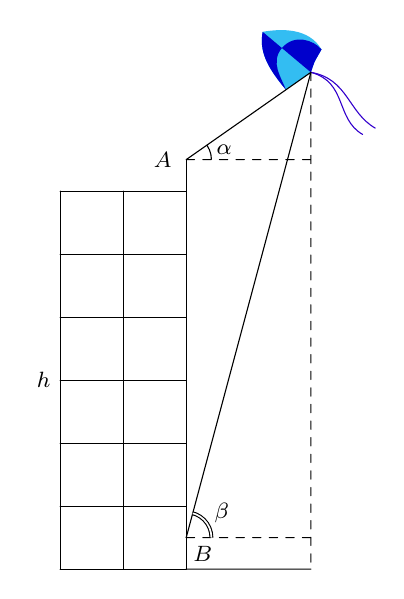
\begin{tikzpicture}[scale=.8,font=\footnotesize,line cap=round,line join=round,>=stealth]
    \draw (0,0) coordinate(O)grid (2,6);
    \draw (2,6)--(2,6.5) coordinate(A) (2,.5) coordinate(B);
    \path[shift={(B)}] (75:1) coordinate(b);
    \path[shift={(A)}] (35:1) coordinate(a);
    \path (intersection of A--a and B--b) coordinate(C) ($(A)!.8!(C)$) coordinate(D) ($(O)!(C)!(5,0)$) coordinate(H) ($(C)!(A)!(H)$) coordinate(I) ($(C)!(B)!(H)$) coordinate(J);
    \path[shift={(C)}] (65:.4) coordinate(E) (140:1) coordinate(F) ($(C)!.6!(F)$) coordinate(G);
    \fill[cyan!80] (C)--(D) .. controls + (130:.5) and +(-100:.3) .. (F) .. controls +(10:.3) and +(120:.4) ..(E) .. controls +(-120:.3) and +(70:.2) .. cycle;
    \fill[blue!80!black] (C)--(G) .. controls +(50:.3) and +(130:.2) .. (E) .. controls +(-120:.3) and +(70:.2) .. cycle;
    \fill[blue!80!black] (D) .. controls + (130:.5) and +(-100:.3) .. (F) -- (G) .. controls +(-130:.3) and +(110:.2) .. cycle;
    \draw[color=blue!80!red] (C) .. controls +(-10:.6) and +(150:.5) .. (5,7);
    \draw[color=blue!80!red] (C) .. controls +(-15:.6) and +(150:.5) .. (4.8,6.9);
    \draw (A)--(C)--(B) (2,0)--(H);
    \draw[dashed] (C)--(H) (A)--(I) (B)--(J);
    \path (O)--(0,6) node[midway,left]{$h$} (A) node[shift={(180:.3)}]{$A$} (B) node[shift={(-45:.3)}]{$B$};
    \begin{scope}
        \clip (C)--(A)--(I);
        \draw (A) circle(.4) node[shift={(15:.5)}]{$\alpha$};
    \end{scope}
    \begin{scope}
        \clip (C)--(B)--(J);
        \draw[double] (B) circle(.4) node[shift={(35:.55)}]{$\beta$};
    \end{scope}
    
\end{tikzpicture}
    
\end{center}
\shortans[oly]{${27,9}$}

\loigiai{ 

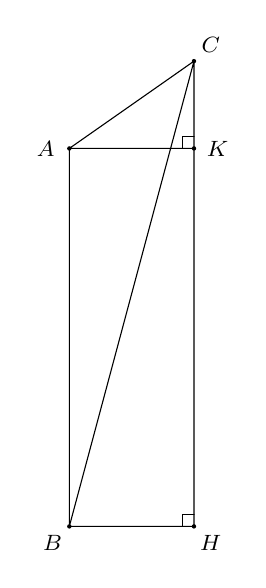
\begin{tikzpicture}[scale=.8,font=\footnotesize,line cap=round,line join=round,>=stealth]
    \path (0,0) coordinate(B) (0,6) coordinate(A) + (35:1) coordinate(a) (75:1) coordinate(b) (intersection of A--a and B--b) coordinate(C) ($(B)!(C)!(1,0)$) coordinate(H) ($(C)!(A)!(H)$) coordinate(K);
    \draw (A)--(B)--(C)--cycle (C)--(H)--(B) (A)--(K);
    \foreach \d/\g in {A/180, B/-135, C/45, H/-45, K/0}
    \fill (\d) circle(1pt) node[shift={(\g:.3)}]{$\d$};
    \path pic[draw,angle radius=.15cm]{right angle=A--K--C} pic[draw,angle radius=.15cm]{right angle=B--H--C};
       
    
\end{tikzpicture}
     
 Kí hiệu ${C}$ là vị trí của chiếc diều.

Từ điểm ${B}$ vẽ đường thẳng $Bx$ vuông góc với ${AB}$.

Từ điểm ${C}$ kẻ $CH\perp Bx$ (${H}$ thuộc ${Bx}$).

Từ điểm ${A}$ kẻ $AK\perp CH$ (${K}$ thuộc ${CH}$).

Khi đó $\widehat{CAK}=\alpha$ và $\widehat{CBH}=\beta$.

Chiều cao của diều so với mặt đất chính là độ dài đoạn thẳng ${CH}$.

Vì khoảng cách từ đỉnh tòa nhà tới mắt bạn ${A}$ và khoảng cách từ mặt đất tới mắt bạn ${B}$ đều là ${1,1}$m nên ${AB=h=21}$m.

Tứ giác ${ABHK}$ là hình chữ nhật.

$\widehat{CAB} = \widehat{CAK}+\widehat{KAB} = 32^{\circ} + 90^{\circ} = 122^{\circ}$.

$\widehat{CBA} = \widehat{ABH}-\widehat{CBH} = 90^{\circ}-71^{\circ} = 19^{\circ}$.

Trong tam giác ${ABC}$ ta có 

$\widehat{C}= 180^{\circ} - \left(\widehat{A}+\widehat{B}\right) = 180^{\circ} - \left(122^{\circ}+19^{\circ}\right) = 39^{\circ}$.

Áp dụng định lí sin trong tam giác ${ABC}$ ta có

$\dfrac{AB}{ \sin C} = \dfrac{BC}{\sin A } \Rightarrow BC = \dfrac{AB\sin A}{\sin C} = \dfrac{ 21\sin 122^{\circ} }{\sin 39^{\circ} } \approx 28$

Trong tam giác ${CBH}$ vuông tại ${H}$ ta có 

$CH=BC\sin B  \approx 28\sin{ 71^{\circ} }\approx 27$ m

Vậy chiếc diều bay cao khoảng ${27,9}$ mét so với mặt đất. 
 }\end{ex}

\Closesolutionfile{ans}

 \begin{center}
-----HẾT-----
\end{center}

 %\newpage 
%\begin{center}
%{\bf BẢNG ĐÁP ÁN MÃ ĐỀ 159 }
%\end{center}
%{\bf Phần 1 }
% \inputansbox{6}{ans159-1}
%{\bf Phần 2 }
% \inputansbox{2}{ans159-2}
%{\bf Phần 3 }
% \inputansbox{6}{ans159-3}
\newpage 




\end{document}